\subsection{Model Architectures}

\begin{frame}{Model Architectures}
    \begin{columns}
        \begin{column}{0.4\textwidth}
            Summarization models are hierarchical with the following
            components:
            \begin{itemize}
                \item Word Embedding Layer
                \item Sentence Encoder Layer
                \item Sentence Extractor Layer
            \end{itemize}
        \end{column}
        \begin{column}{0.58\textwidth}
      \resizebox{\textwidth}{!}{
    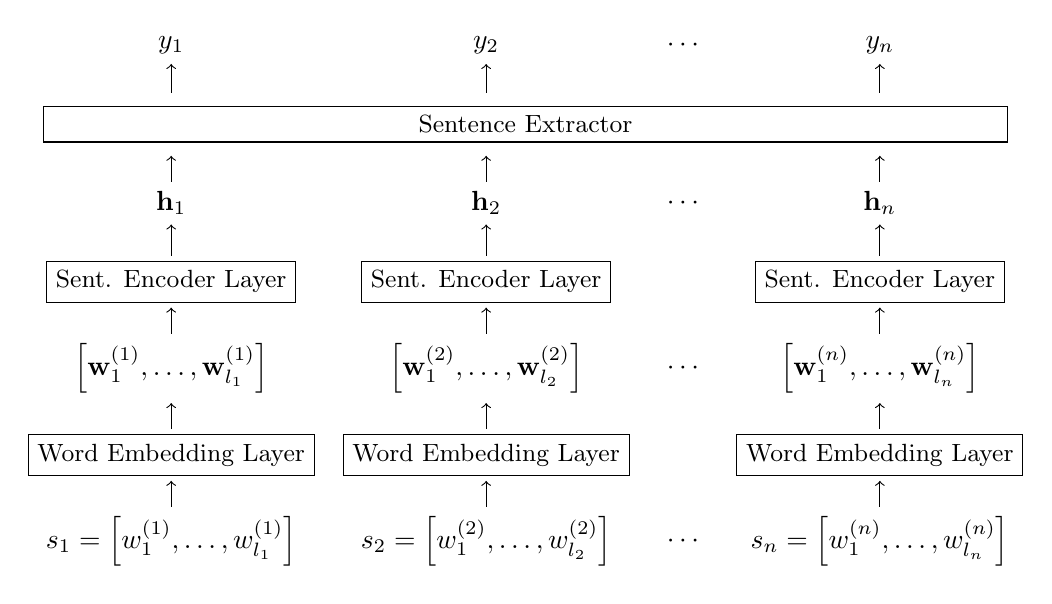
\begin{tikzpicture}[
            emb/.style={draw,font=\small,outer sep=2pt},
        ]
    \node (s1) at (0,0)  {$s_1=\left[w_1^{(1)},\ldots,w_{l_1}^{(1)}\right]$};
    \node[emb] (embl1) at (0,1.10)  {Word Embedding Layer};
    \draw[->] (s1.north) -- (embl1.south);
    \node (emb1) at (0,2.2) {$\left[\mathbf{w}_1^{(1)},\ldots,\mathbf{w}_{l_1}^{(1)}\right]$};
    \draw[->] (embl1.north) -- (emb1.south);
    \node[emb] (encl1) at (0,3.3)  {Sent. Encoder Layer};
    \draw[->] (emb1.north) -- (encl1.south);
    \node (enc1) at (0,4.3) {$\mathbf{h}_1$};
    \draw[->] (encl1.north) -- (enc1.south);

    \node (s2) at (4,0)  {$s_2=\left[w_1^{(2)},\ldots,w_{l_2}^{(2)}\right]$};
    \node[emb] (embl2) at (4,1.1)  {Word Embedding Layer};
    \draw[->] (s2.north) -- (embl2.south);
    \node (emb2) at (4,2.2) {$\left[\mathbf{w}_1^{(2)},\ldots,\mathbf{w}_{l_2}^{(2)}\right]$};
    \draw[->] (embl2.north) -- (emb2.south);
    \node[emb] (encl2) at (4,3.3)  {Sent. Encoder Layer};
    \draw[->] (emb2.north) -- (encl2.south);
    \node (enc2) at (4,4.3) {$\mathbf{h}_2$};
    \draw[->] (encl2.north) -- (enc2.south);
    
    \node (sn) at (9.0,0)  {$s_n=\left[w_1^{(n)},\ldots,w_{l_n}^{(n)}\right]$};
    \node[emb] (embln) at (9,1.1)  {Word Embedding Layer};
    \draw[->] (sn.north) -- (embln.south);
    \node (embn) at (9,2.2) {$\left[\mathbf{w}_1^{(n)},\ldots,\mathbf{w}_{l_n}^{(n)}\right]$};
    \draw[->] (embln.north) -- (embn.south);
    \node[emb] (encln) at (9,3.3)  {Sent. Encoder Layer};
    \draw[->] (embn.north) -- (encln.south);
    \node (encn) at (9,4.3) {$\mathbf{h}_n$};
    \draw[->] (encln.north) -- (encn.south);
    \draw[->] (encn.north) -- (9,4.9);
    \draw[->] (enc2.north) -- (4,4.9);
    \draw[->] (enc1.north) -- (0,4.9);
    \node[emb,text width=12cm,align=center] at (4.5,5.3) {Sentence Extractor};

    \node at (6.5,0)  {$\large \cdots$};
    \node at (6.5,2.2)  {$\large \cdots$};
    \node at (6.5,4.3)  {$\large \cdots$};

    \node (y1) at (0,6.3) {$y_1$};
    \draw[->] (0,5.7) -- (y1.south);
    \node (y2) at (4,6.3) {$y_2$};
    \draw[->] (4,5.7) -- (y2.south);
    \node (yel) at (6.5,6.3)  {$\cdots$};
    \node (y3) at (9,6.3) {$y_n$};
    \draw[->] (9,5.7) -- (y3.south);
\end{tikzpicture}}
\end{column}
\end{columns}
\end{frame}


\begin{frame}{Sentence Encoders/Extractors}

    \begin{itemize}
        \item We compare 3 different Sentence Encoder Layers:
            \begin{itemize}
                \item Averaging Encoder
                \item CNN Encoder 
                \item RNN Encoder
                \end{itemize}
            \vspace{5pt}
        \item We compare two prior Sentence Extractor Layers,
                SummaRunner Extractor {\tiny (Nallapati et al., 2016)}
                and  Cheng \& Lapata Extractor {\tiny(Cheng and Lapata, 2016)}
                \begin{itemize}
                    \item (SummaRunner only) Internal vector represenatations of summary and document constructed from sentence embeddings.
                    \item Models dependencies between earlier predictions
                        and subsequent predictions.
                \end{itemize}
            \vspace{5pt}
       \item We propose a variant of each Sentence Extractor with less task 
           specific architecture using common neural network components.
            \begin{itemize}
                \item RNN Extractor -- biRNN tagger
                \item Seq2Seq Extractor -- seq2seq with attention
                \begin{itemize}
                    \item No internal represenatations of summary/document.
                    \item Dependencies between predictions not modeled.
            \end{itemize}
            \end{itemize}
    \end{itemize}

\end{frame}


